%%%%%%%%%%%%%%%%%%%%%%%%%%%%%%%%%%%%%%%%%%%%%%%%%%%%%%%%%%%%%%%
%
% Welcome to writeLaTeX --- just edit your LaTeX on the left,
% and we'll compile it for you on the right. If you give
% someone the link to this page, they can edit at the same
% time. See the help menu above for more info. Enjoy!
%
%%%%%%%%%%%%%%%%%%%%%%%%%%%%%%%%%%%%%%%%%%%%%%%%%%%%%%%%%%%%%%%

% --------------------------------------------------------------
% This is all preamble stuff that you don't have to worry about.
% Head down to where it says "Start here"
% --------------------------------------------------------------
 
\documentclass[12pt]{article}
 
\usepackage[margin=1in]{geometry}
\usepackage{amsmath,amsthm,amssymb}

\usepackage{listings}
\usepackage{xcolor}

\usepackage{tikz}
\usetikzlibrary{shapes,positioning}

\tikzset{ell/.style={circle,draw,minimum height=0.5cm,minimum width=0.5cm,inner sep=0.2cm}}

%New colors defined below
\definecolor{codegreen}{rgb}{0,0.6,0}
\definecolor{codegray}{rgb}{0.5,0.5,0.5}
\definecolor{codepurple}{rgb}{0.58,0,0.82}
\definecolor{backcolour}{rgb}{0.95,0.95,0.92}

%Code listing style named "mystyle"
\lstdefinestyle{mystyle}{
  backgroundcolor=\color{backcolour}, commentstyle=\color{codegreen},
  keywordstyle=\color{magenta},
  numberstyle=\tiny\color{codegray},
  stringstyle=\color{codepurple},
  basicstyle=\ttfamily\footnotesize,
  breakatwhitespace=false,         
  breaklines=true,                 
  captionpos=b,                    
  keepspaces=true,                 
  numbers=left,                    
  numbersep=5pt,                  
  showspaces=false,                
  showstringspaces=false,
  showtabs=false,                  
  tabsize=2
}

%"mystyle" code listing set
\lstset{style=mystyle}

 
\newcommand{\N}{\mathbb{N}}
\newcommand{\Z}{\mathbb{Z}}
 
\newenvironment{theorem}[2][Theorem]{\begin{trivlist}
\item[\hskip \labelsep {\bfseries #1}\hskip \labelsep {\bfseries #2.}]}{\end{trivlist}}
\newenvironment{lemma}[2][Lemma]{\begin{trivlist}
\item[\hskip \labelsep {\bfseries #1}\hskip \labelsep {\bfseries #2.}]}{\end{trivlist}}
\newenvironment{exercise}[2][Exercise]{\begin{trivlist}
\item[\hskip \labelsep {\bfseries #1}\hskip \labelsep {\bfseries #2.}]}{\end{trivlist}}
\newenvironment{problem}[2][Problem]{\begin{trivlist}
\item[\hskip \labelsep {\bfseries #1}\hskip \labelsep {\bfseries #2.}]}{\end{trivlist}}
\newenvironment{question}[2][Question]{\begin{trivlist}
\item[\hskip \labelsep {\bfseries #1}\hskip \labelsep {\bfseries #2.}]}{\end{trivlist}}
\newenvironment{corollary}[2][Corollary]{\begin{trivlist}
\item[\hskip \labelsep {\bfseries #1}\hskip \labelsep {\bfseries #2.}]}{\end{trivlist}}

\newenvironment{solution}{\begin{proof}[Solution]}{\end{proof}}
 
\begin{document}
 
% --------------------------------------------------------------
%                         Start here
% --------------------------------------------------------------
 
\title{Discussion 8}%replace X with the appropriate number
\author{Mengxiang Jiang\\ %replace with your name
CSEN 5303 Foundations of Computer Science} %if necessary, replace with your course title
 
\maketitle

\begin{problem}{statement}
  Feel free to discuss one (1) of the following topics.\\
1. Tree traversal algorithms\\
2. Spanning tree\\
3. Minimum spanning tree\\
4. Depth-first search\\
5. Breadth-first search\\
6. Kruskal's algorithm\\
7. Prim's algorithm\\
\end{problem}

\begin{problem}{1} %You can use theorem, exercise, problem, or question here.  Modify x.yz to be whatever number you are proving
There are three main tree traversal algorithms: $preorder$, $inorder$, and $postorder$.\\
These three methods are defined with ``traverse'' meaning recursively calling the method:
\begin{quote}
  Preorder\\
  Visit the root\\
  Traverse the leftmost subtree\\
  Traverse the 2nd leftmost subtree\\
  ...\\
  Traverse the rightmost subtree
\end{quote}

\begin{quote}
  Inorder\\
  Traverse the leftmost subtree\\
  Visit the root\\
  Traverse the 2nd leftmost subtree\\
  ...\\
  Traverse the rightmost subtree
\end{quote}

\begin{quote}
  Postorder\\
  Traverse the leftmost subtree\\
  Traverse the 2nd leftmost subtree\\
  ...\\
  Traverse the rightmost subtree\\
  Visit the root
\end{quote}

\pagebreak
Below is a tree that will be used to illustrate the different traversal algorithms:\\

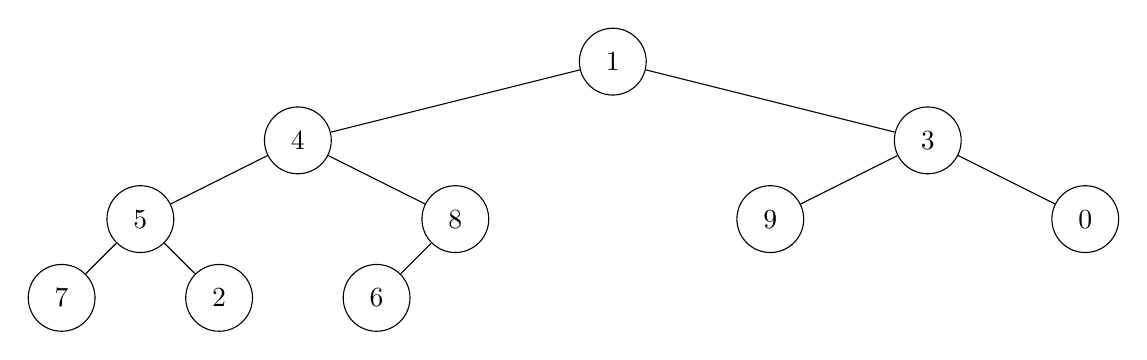
\begin{tikzpicture}[>=stealth]
  \node[ell] (a)at (8,3) {1};
  \node[ell] (b)at (4,2) {4};
  \node[ell] (c)at (12,2) {3};
  \node[ell] (d)at (2,1) {5};
  \node[ell] (e)at (6,1) {8};
  \node[ell] (f)at (10,1) {9};
  \node[ell] (g)at (14,1) {0};
  \node[ell] (h)at (1,0) {7};
  \node[ell] (i)at (3,0) {2};
  \node[ell] (j)at (5,0) {6};

  \draw [] (a) to []node[]{} (b);
  \draw [] (a) to []node[]{} (c);
  \draw [] (b) to []node[]{} (d);
  \draw [] (b) to []node[]{} (e);
  \draw [] (c) to []node[]{} (f);
  \draw [] (c) to []node[]{} (g);
  \draw [] (d) to []node[]{} (h);
  \draw [] (d) to []node[]{} (i);
  \draw [] (e) to []node[]{} (j);
\end{tikzpicture}
\linebreak
For preorder, the order the nodes that a visited are 1, 4, 5, 7, 2, 8, 6, 3, 9, 0\\
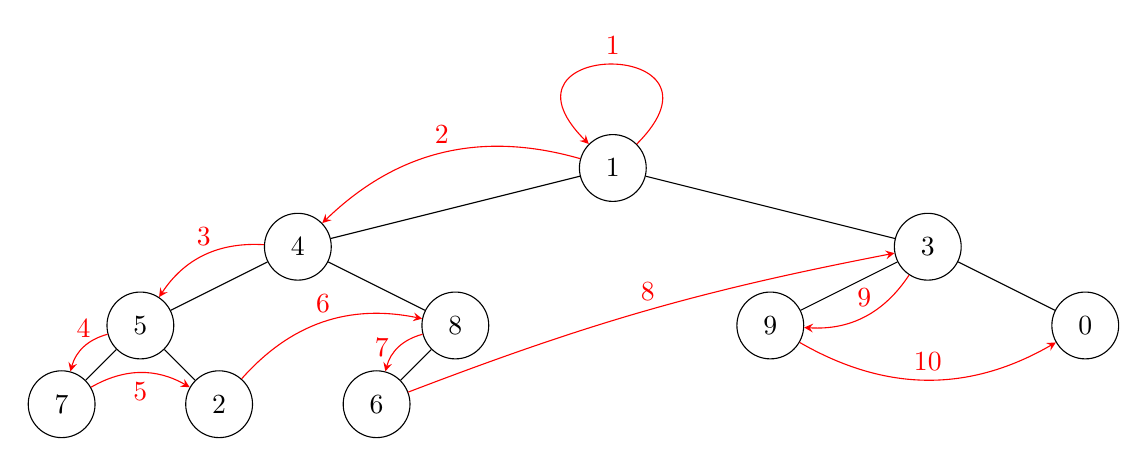
\begin{tikzpicture}[>=stealth]
  \node[ell] (a)at (8,3) {1};
  \node[ell] (b)at (4,2) {4};
  \node[ell] (c)at (12,2) {3};
  \node[ell] (d)at (2,1) {5};
  \node[ell] (e)at (6,1) {8};
  \node[ell] (f)at (10,1) {9};
  \node[ell] (g)at (14,1) {0};
  \node[ell] (h)at (1,0) {7};
  \node[ell] (i)at (3,0) {2};
  \node[ell] (j)at (5,0) {6};

  \draw [red,->] (a) to [loop]node[above]{1} (a);
  \draw [] (a) to []node[]{} (b);
  \draw [red,->] (a) to [bend right]node[above]{2} (b);
  \draw [] (a) to []node[]{} (c);
  \draw [] (b) to []node[]{} (d);
  \draw [red,->] (b) to [bend right]node[above]{3} (d);
  \draw [] (b) to []node[]{} (e);
  \draw [] (c) to []node[]{} (f);
  \draw [] (c) to []node[]{} (g);
  \draw [] (d) to []node[]{} (h);
  \draw [red,->] (d) to [bend right]node[above]{4} (h);
  \draw [] (d) to []node[]{} (i);
  \draw [red,->] (h) to [bend left]node[below]{5} (i);
  \draw [red,->] (i) to [bend left]node[above]{6} (e);
  \draw [] (e) to []node[]{} (j);
  \draw [red,->] (e) to [bend right]node[left]{7} (j);
  \draw [red,->] (j) to [bend left=5]node[above]{8} (c);
  \draw [red,->] (c) to [bend left]node[above]{9} (f);
  \draw [red,->] (f) to [bend right]node[above]{10} (g);
\end{tikzpicture}
\linebreak
For inorder, the order the nodes that are visited are 7, 5, 2, 4, 6, 8, 1, 9, 3, 0\\
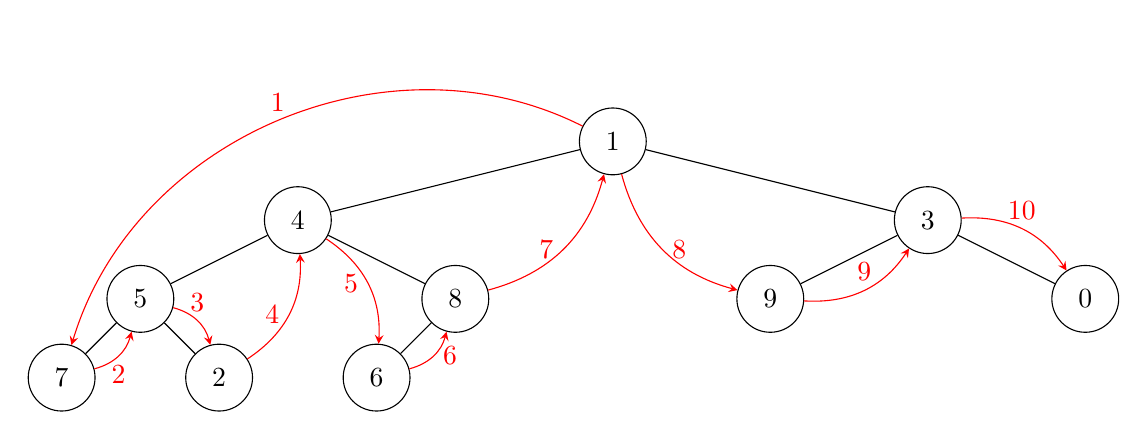
\begin{tikzpicture}[>=stealth]
  \node[ell] (a)at (8,3) {1};
  \node[ell] (b)at (4,2) {4};
  \node[ell] (c)at (12,2) {3};
  \node[ell] (d)at (2,1) {5};
  \node[ell] (e)at (6,1) {8};
  \node[ell] (f)at (10,1) {9};
  \node[ell] (g)at (14,1) {0};
  \node[ell] (h)at (1,0) {7};
  \node[ell] (i)at (3,0) {2};
  \node[ell] (j)at (5,0) {6};

  \draw [red,->] (a) to [bend right=50]node[above]{1} (h);
  \draw [] (a) to []node[]{} (b);
  \draw [red,->] (h) to [bend right]node[below]{2} (d);
  \draw [] (a) to []node[]{} (c);
  \draw [] (b) to []node[]{} (d);
  \draw [red,->] (d) to [bend left]node[above]{3} (i);
  \draw [] (b) to []node[]{} (e);
  \draw [] (c) to []node[]{} (f);
  \draw [] (c) to []node[]{} (g);
  \draw [] (d) to []node[]{} (h);
  \draw [red,->] (i) to [bend right]node[left]{4} (b);
  \draw [] (d) to []node[]{} (i);
  \draw [red,->] (b) to [bend left]node[left]{5} (j);
  \draw [red,->] (j) to [bend right]node[right]{6} (e);
  \draw [] (e) to []node[]{} (j);
  \draw [red,->] (e) to [bend right]node[left]{7} (a);
  \draw [red,->] (a) to [bend right]node[right]{8} (f);
  \draw [red,->] (f) to [bend right]node[above]{9} (c);
  \draw [red,->] (c) to [bend left]node[above]{10} (g);
\end{tikzpicture}
\linebreak
For postorder, the order the nodes that are visited are 7, 2, 5, 6, 8, 4, 9, 0, 3, 1\\
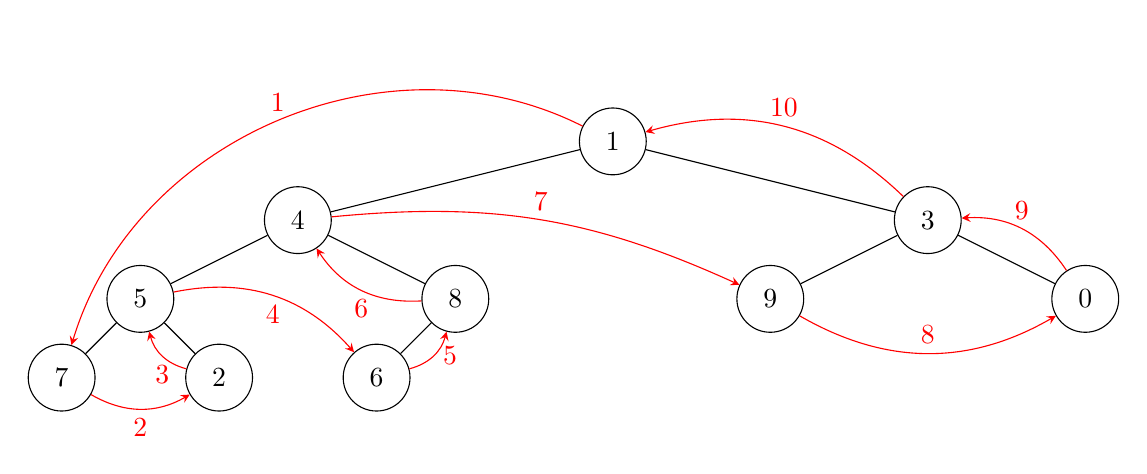
\begin{tikzpicture}[>=stealth]
  \node[ell] (a)at (8,3) {1};
  \node[ell] (b)at (4,2) {4};
  \node[ell] (c)at (12,2) {3};
  \node[ell] (d)at (2,1) {5};
  \node[ell] (e)at (6,1) {8};
  \node[ell] (f)at (10,1) {9};
  \node[ell] (g)at (14,1) {0};
  \node[ell] (h)at (1,0) {7};
  \node[ell] (i)at (3,0) {2};
  \node[ell] (j)at (5,0) {6};

  \draw [red,->] (a) to [bend right=50]node[above]{1} (h);
  \draw [] (a) to []node[]{} (b);
  \draw [red,->] (h) to [bend right]node[below]{2} (i);
  \draw [] (a) to []node[]{} (c);
  \draw [] (b) to []node[]{} (d);
  \draw [red,->] (i) to [bend left]node[below]{3} (d);
  \draw [] (b) to []node[]{} (e);
  \draw [] (c) to []node[]{} (f);
  \draw [] (c) to []node[]{} (g);
  \draw [] (d) to []node[]{} (h);
  \draw [red,->] (d) to [bend left]node[below]{4} (j);
  \draw [] (d) to []node[]{} (i);
  \draw [red,->] (j) to [bend right]node[right]{5} (e);
  \draw [red,->] (e) to [bend left]node[below]{6} (b);
  \draw [] (e) to []node[]{} (j);
  \draw [red,->] (b) to [bend left=15]node[above]{7} (f);
  \draw [red,->] (f) to [bend right]node[above]{8} (g);
  \draw [red,->] (g) to [bend right]node[above]{9} (c);
  \draw [red,->] (c) to [bend right]node[above]{10} (a);
\end{tikzpicture}

\end{problem}
% --------------------------------------------------------------
%     You don't have to mess with anything below this line.
% --------------------------------------------------------------
 
\end{document}